\subsection{Graphismes}

Pour rendre le jeu plus beau, nous avons intégré plusieurs effets.
Afin de les créer, nous avons utilisé plusieurs outils de Unity :
Shader Graph, TimeLine, Visual Effect FX Graph, Cinemachine.

Voici plusieurs exemples des éléments graphiques que nous avons pu réaliser : 


\subsubsection{Shader Eau}

L'eau que nous avions était plate mais surtout n'était pas animée.
Plutôt que d'acheter un asset permettant d'avoir de l'eau animée,
nous avons opté pour une réalisation manuelle à l'aide de l'outil Shader Graph.

Il y a trois blocs pour les vagues (les petites, les moyennes et les grandes),
ainsi que des blocs sinusoïdaux pour que chaque bloc d'eau soit aligné et synchronisé avec les autres.
\begin{figure}[hbt!]
    \centering
    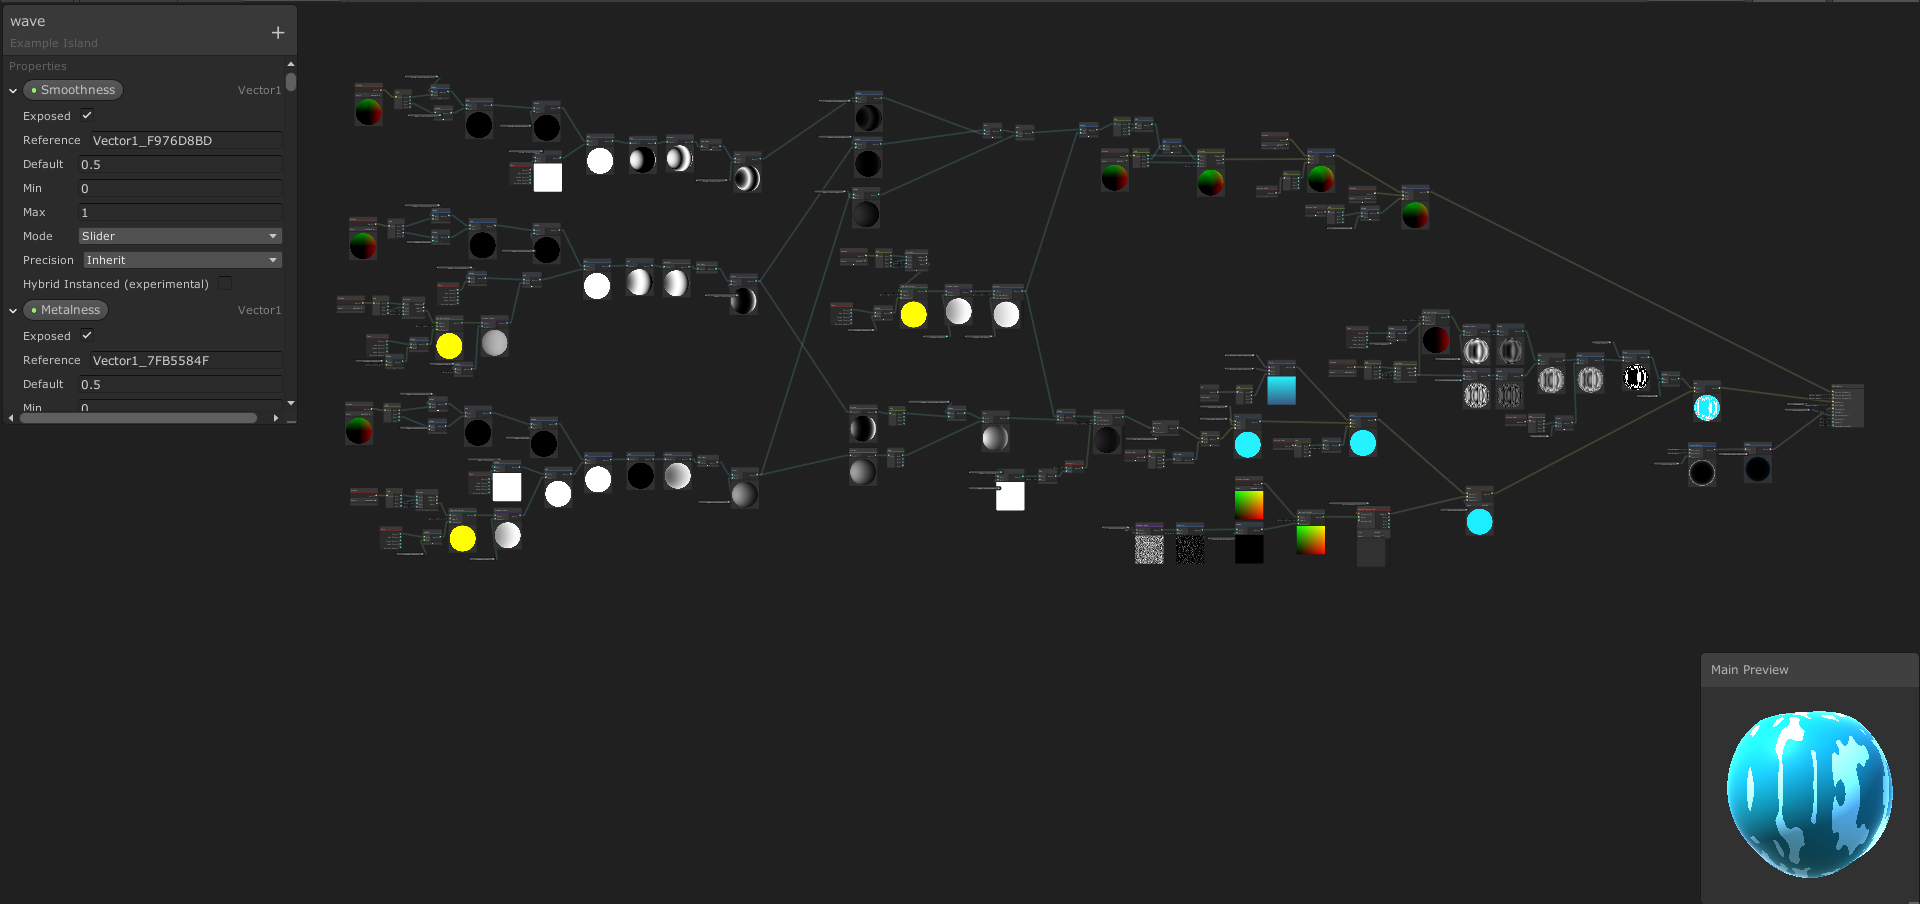
\includegraphics[scale=0.2]{waterShaderGraph.png}
    \caption{Shader Graph de l'eau}
\end{figure}
\begin{figure}[hbt!]
    \centering
    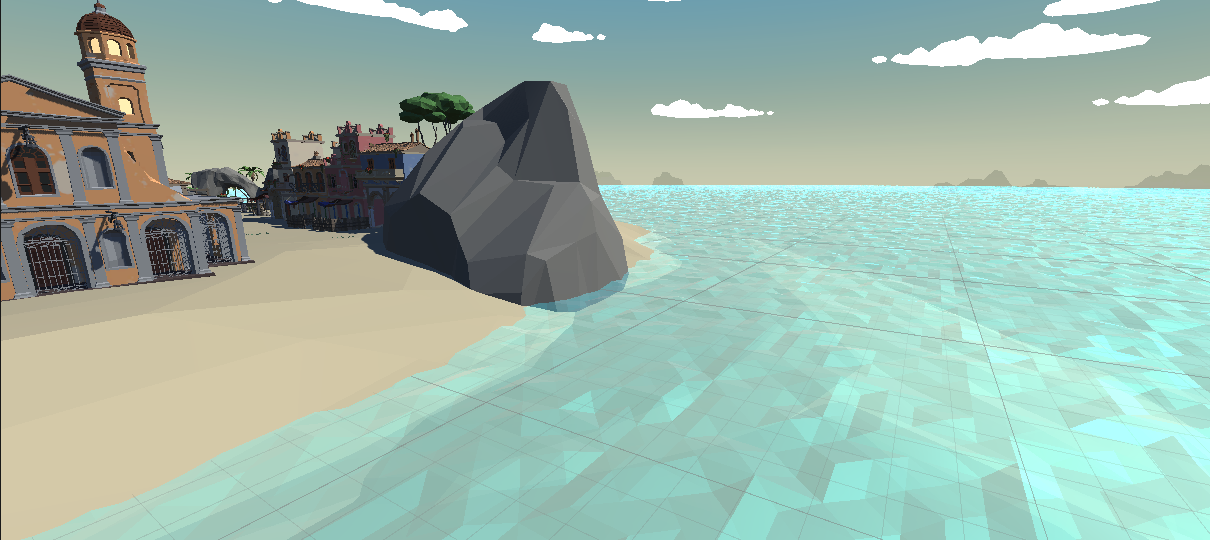
\includegraphics[scale=0.3]{waterBefore.png}
    \caption{L'eau avant}
    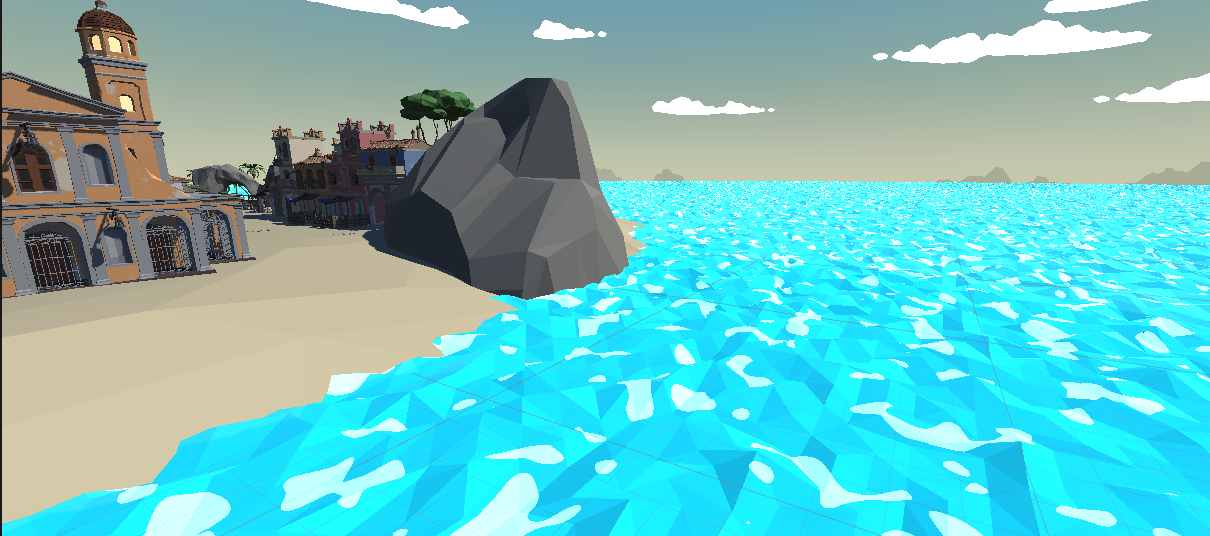
\includegraphics[scale=0.3]{WaterAfter.png}
    \caption{L'eau après}
\end{figure}
\FloatBarrier



\subsubsection{Mode Jour/Nuit}
Le mode jour/nuit permet, au lancement de la partie,
de choisir soit le jour soit la nuit. Si l'on choisit le mode nuit, un script désactive la lampe de jour,
 pour la remplacer par une autre plus sombre. Des effets de pluie ont été rajoutés en plus d'effets de post processing.
Mais l'effet le plus important est d'activer toutes les lampes de la carte.
\begin{figure}[hbt!]
    \centering
    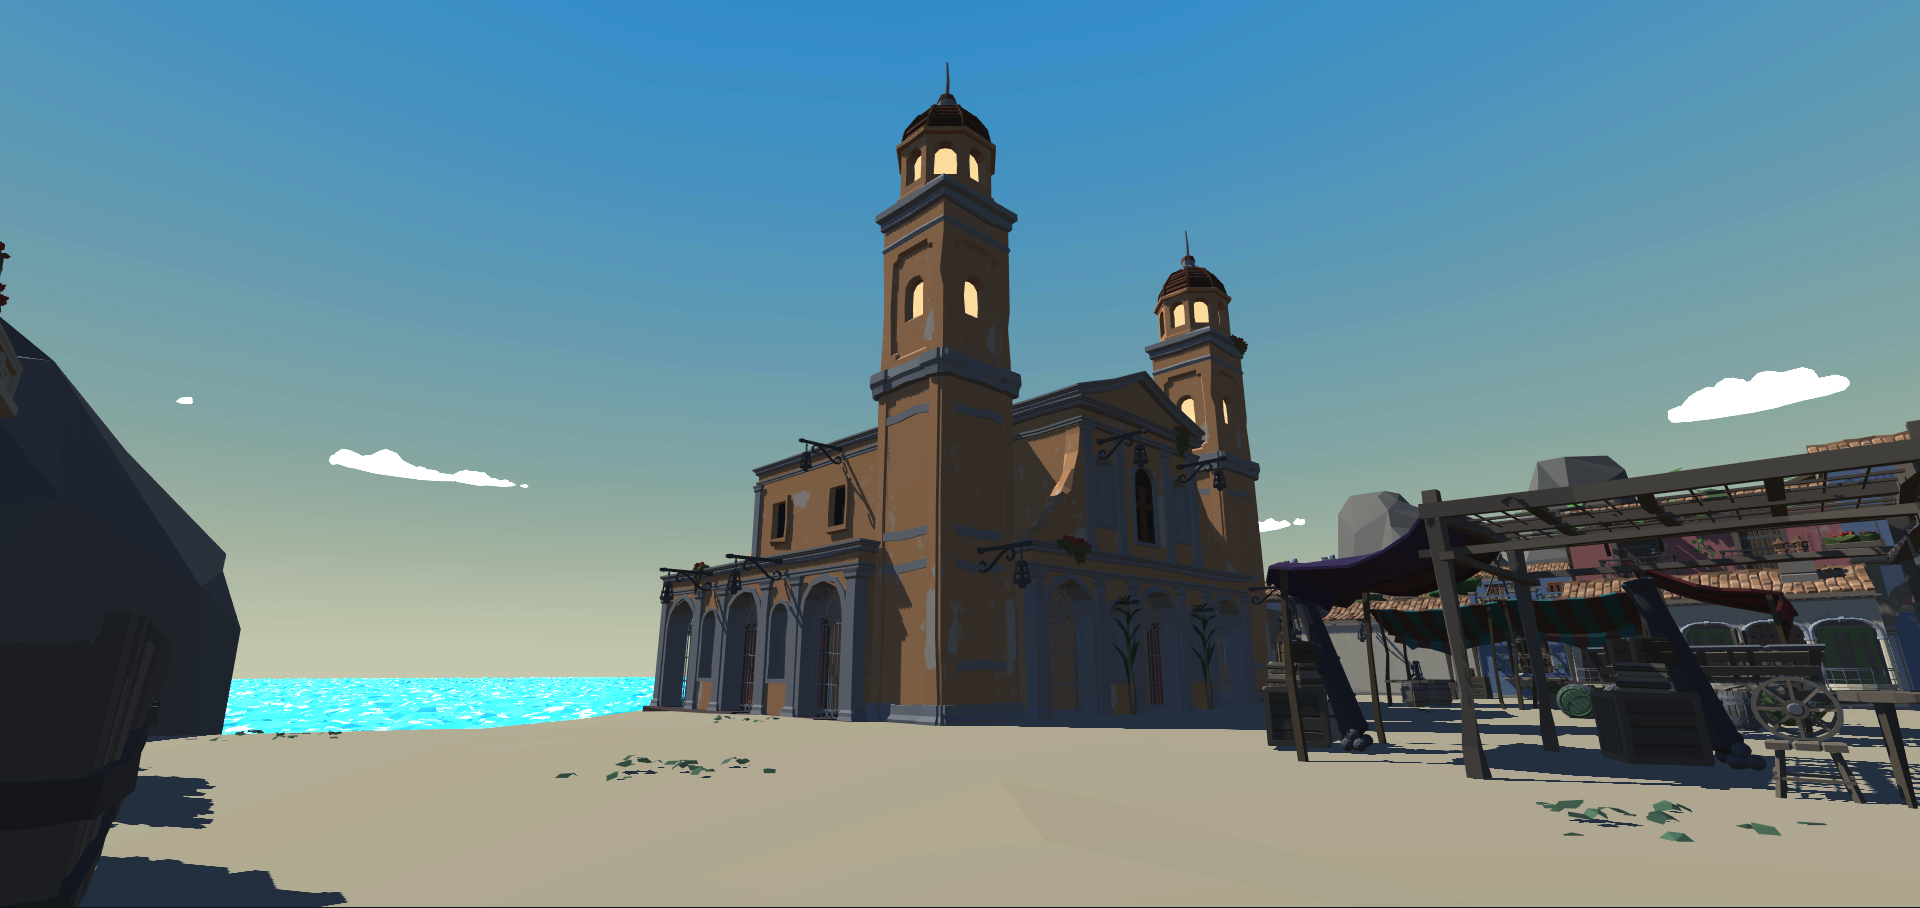
\includegraphics[scale=0.3]{day.png}
    \caption{La carte de jour...}

    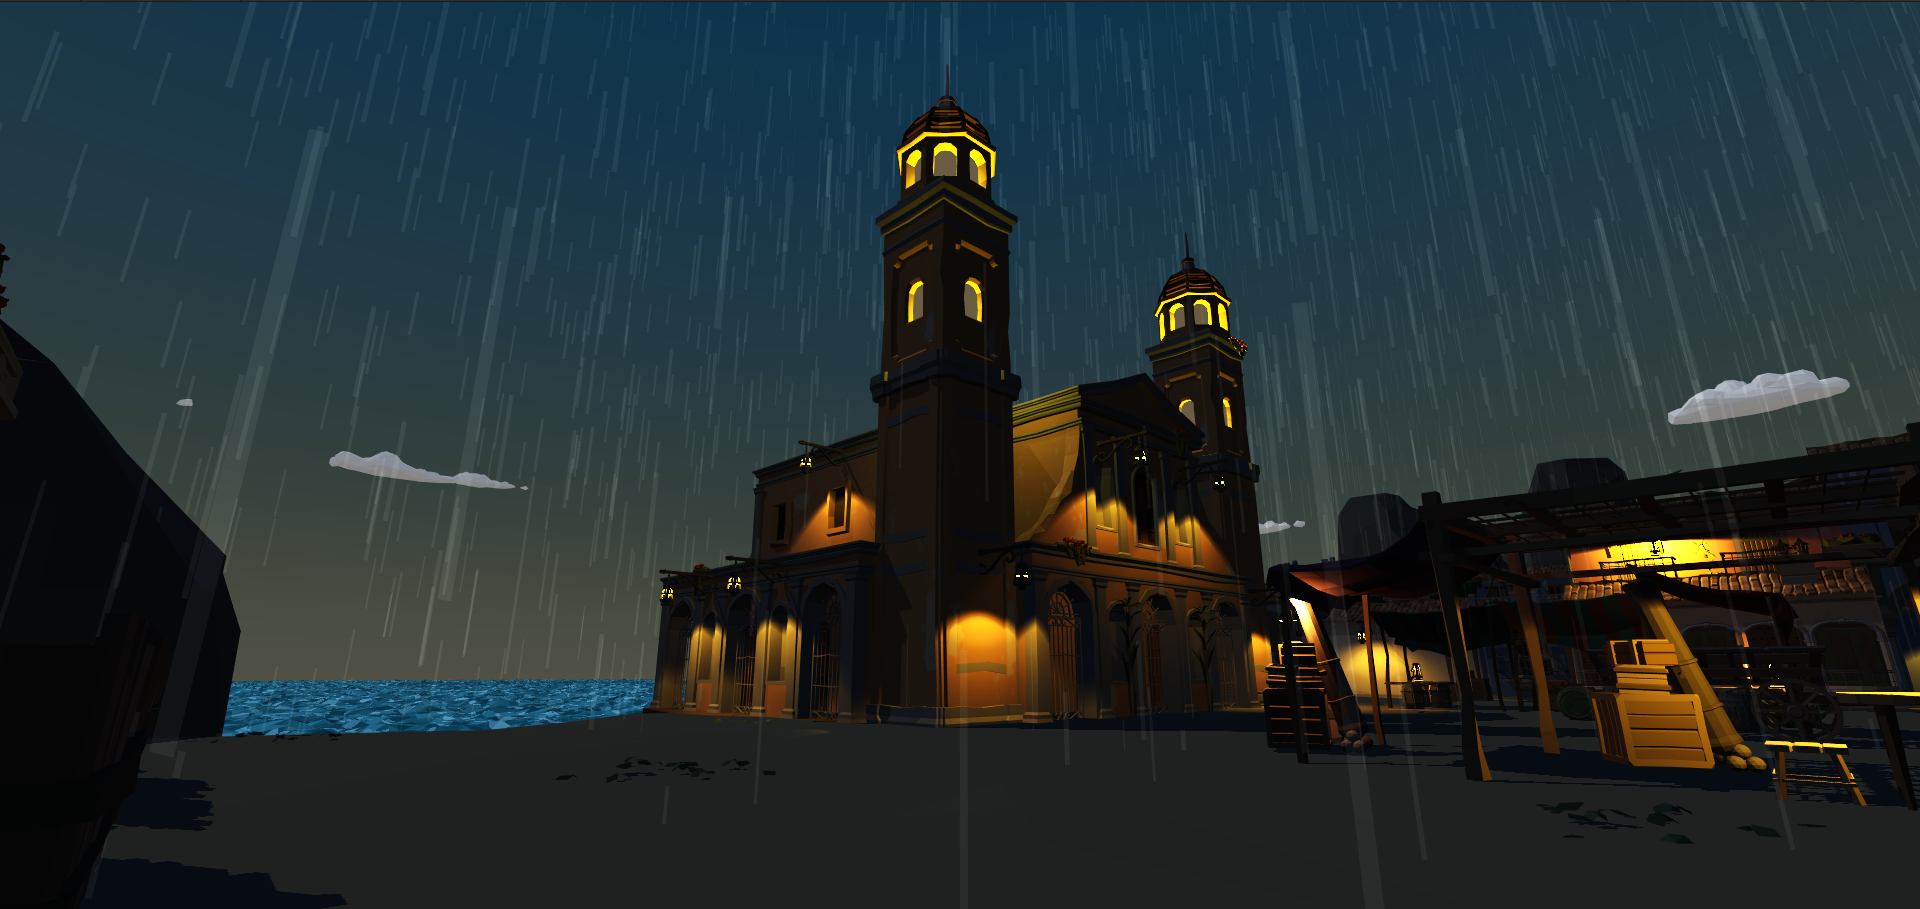
\includegraphics[scale=0.3]{night.png}
    \caption{...et de nuit.}

\end{figure}

\subsubsection{Shader de disparition/apparition}
Pour éviter de faire apparaître ou faire disparaitre en un instant les personnages, nous avons décidé de créer un shader qui qui selon un matériau en paramètre, 
fait une transition de l'état initial vers l'état final. 
\begin{figure}[hbt!]
    \centering
    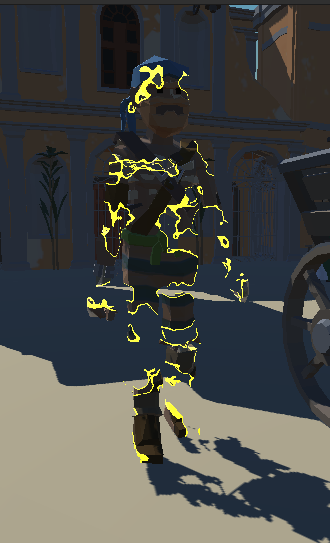
\includegraphics[scale=0.5]{dissolve.png}
    \caption{Application du shader sur un personnage}

\end{figure}
\FloatBarrier

Nous avons rencontré un problème lorsque nous appliquions le matériau avec le shader,
les paramètres de l'instance du shader sur le matériau étant communs. Ainsi, lorsqu'un premier personnage mourrait juste après un autre, 
le premier mort recommençait l'animation de transition en plus de changer de couleur de vêtements et de peau.
La solution trovée, toute simple, consiste à créer un nouveau matériau et d'appliquer  ses paramètres dans le script.

% \subsubsection{Radar}

% A écrire

\subsubsection{Post Processing}

Nous avons ajouté le package Post Processing de Unity qui avec l'URP (Universal Render Pipeline)
nous a permis de créer des ambiances et effets visuels agréables.
Nous avons créé des volumes qui activent les effets de caméra.
Cela nous a permis notamment d'avoir un effet vieux film/sépia lorsque le joueur passe en mode verrouillage.

\begin{figure}[hbt!]
    \centering
    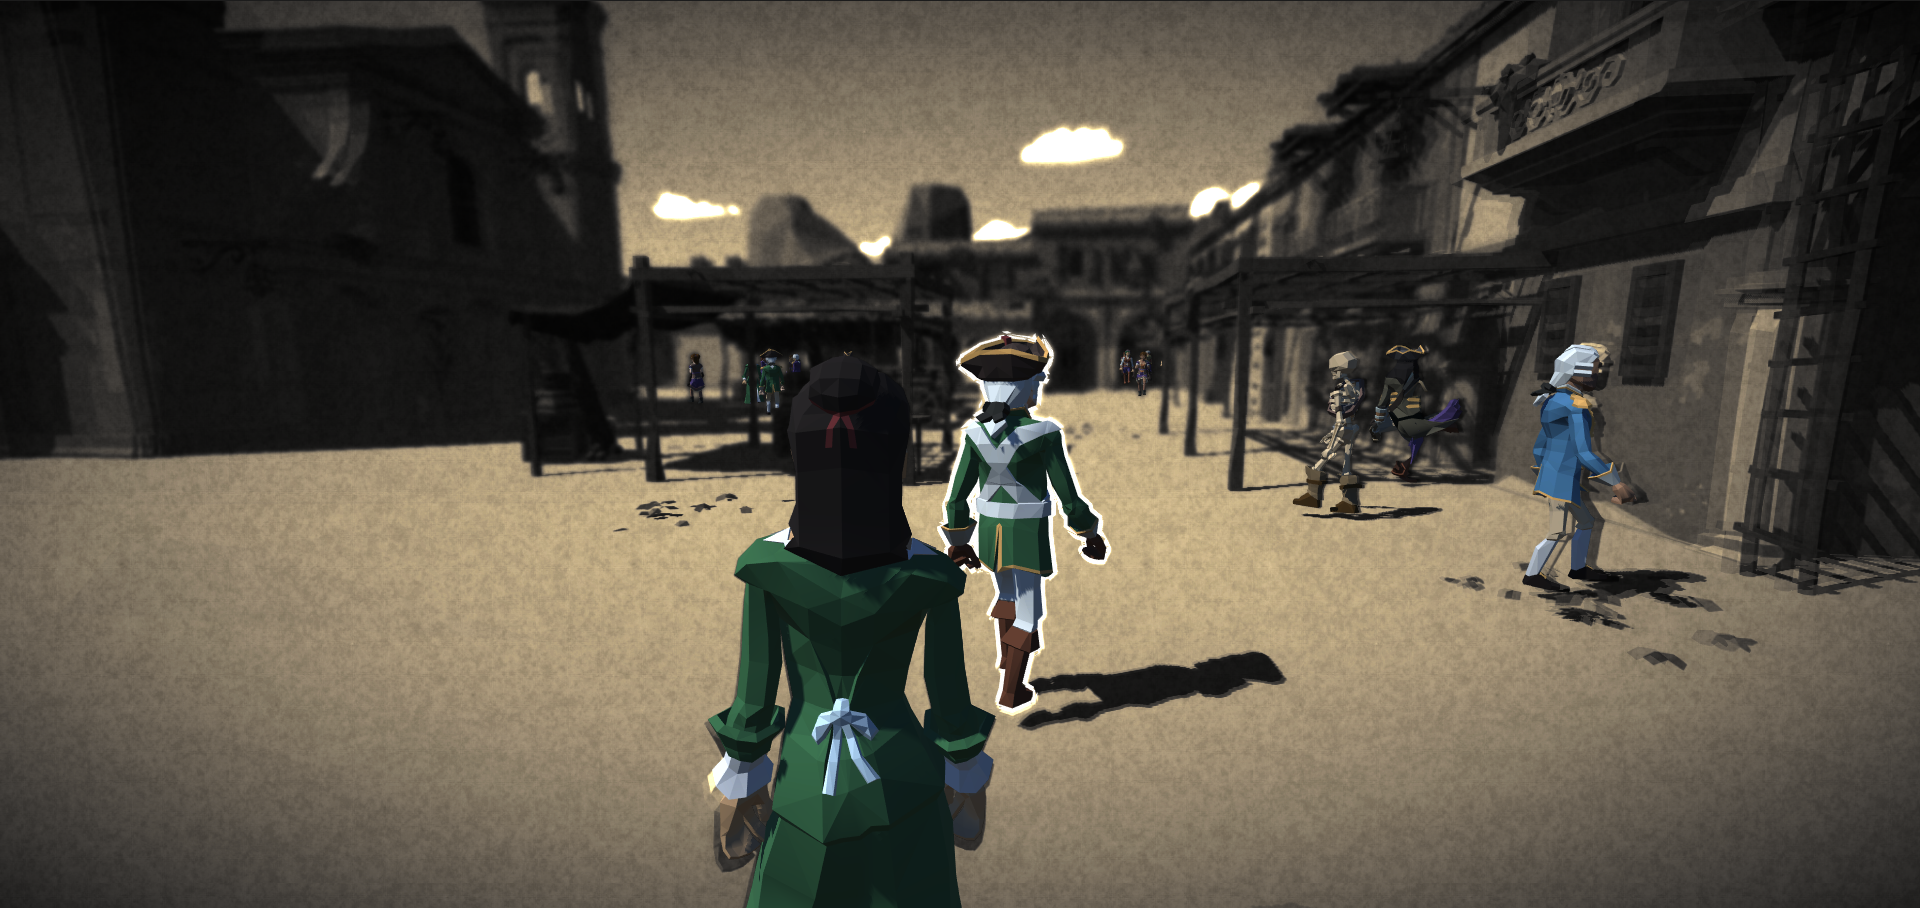
\includegraphics[scale=0.2]{sepia_mode.png}
    \caption{Mode verrouillage}
\end{figure}
\FloatBarrier


Si l'on s'attarde sur cette figure, nous voyons que l'effet "sépia" n'est pas visible sur certains objets.
C'est là toute la difficulté d'avoir des effets de Post Processing différents sur chaque couche.
Nous avons donc ajouté plusieurs caméras \texttt{Overlay} superposées sur la caméra principale qui affichent chacune une partie de l'image.
Après avoir réglé des soucis de profondeur sur les caméras, nous avons obtenu l'effet précédent.